%%%%%%%%%%%%%%%%%%%%%%%%%%%%%%%%%%%%%%
%%%%%%%%%%%%%%%%%%%%%%%%%%%%%%%%%%%%%%
% Do not edit the TeX file your work
% will be overwritten.  Edit the RnW
% file instead.
%%%%%%%%%%%%%%%%%%%%%%%%%%%%%%%%%%%%%%
%%%%%%%%%%%%%%%%%%%%%%%%%%%%%%%%%%%%%%



We demonstrate the local sensitivity computations on a
Gaussian mixture model (GMM) of Fisher's iris data set.
The data set is a sample of 150 iris flowers with
four measurements taken per flower:
sepal length, sepal width, petal length, and petal width.
The GMM was detailed in \exref{iris_bnp_process}; here, the
data dimension $d = 4$. The variational approximation is 
mean-field as in \eqref{vb_mf}, and
we set the truncation parameter $\kmax = 15$.
The variational distribution on all latent variables were taken to 
be the conditionally conjugate (\exref{iris_var_distr}), 
except for the stick-breaking proportions $\nu_\k$ which are logit-normal.

We will investigate how prior choices affect the estimated number of clusters. 
The expected number of \textit{in-sample} clusters $\gclustersabbr$ was defined 
in \exref{vb_insample_nclusters_simple}. 
We will also consider the \textit{posterior predictive} number of clusters, 
\begin{align*}
  \gclusterspredabbr(\eta) &:= \expect{\q(\pi\vert\eta)}{\expect{\p(\z\vert\pi)}{\nclusters(\z)}} \\
  &= \expect{\q(\pi\vert\eta)}{\sum_{k=1}^\kmax\left(1 -
  (1 - \pi_k)^\N \right)}.
\end{align*}
In the iris example, the predictive quantity 
can interpreted as the expected number of species
one might see if a fresh sample of iris flowers were collected.

\todo{make sure this the notation matches from before. }

\subsubsection*{Parametric sensitivity}

We explore how the posterior number of clusters,
either insample or predictive, varies with different choices
of the GEM parameter $\alpha$.
The \textit{a priori} expected number of clusters under a GEM is
\begin{align}\eqlabel{prior_num_clusters}
\sum_{\n = 1}^\N \frac{\alpha}{\alpha + \n - 1},
\end{align}
where $\N$ is the number of observations \citep{jordan:2015:gentleintrodp}.

For the iris data set, we
consider the range $\alpha\in[0.1, 4.0]$.
Using \eqref{prior_num_clusters},
the prior number of clusters is $\approx 1.5$ when $\alpha = 0.1$ and
$\approx 15$ when $\alpha = 4.0$.
The shape of the stick-breaking density varies
considerably for this range of $\alpha$ (\figref{beta_priors}),
and without knowing the true number of iris species, 
it may be unclear which $\alpha$ to choose.


\begin{knitrout}
\definecolor{shadecolor}{rgb}{0.969, 0.969, 0.969}\color{fgcolor}\begin{figure}[!h]

{\centering 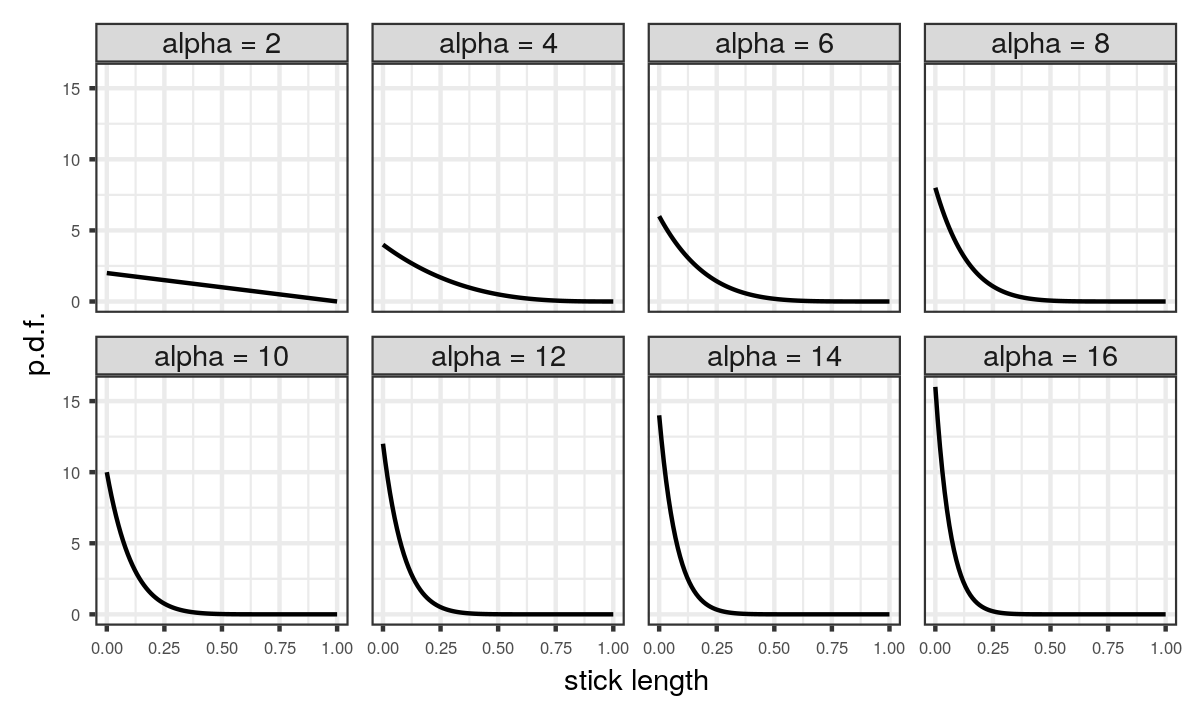
\includegraphics[width=0.980\linewidth,height=0.392\linewidth]{figure/beta_priors-1} 

}

\caption[Probability density functions of $\text{Beta}(1, \alpha)$ distributions, under various $\alpha$ considered for the iris data set]{Probability density functions of $\text{Beta}(1, \alpha)$ distributions, under various $\alpha$ considered for the iris data set.}\label{fig:beta_priors}
\end{figure}


\end{knitrout}


We arbitrarily pick $\alpha_0 = 2$, near the midpoint of our considered range, and
\figref{iris_fit} shows the GMM fit with this prior choice.
The BNP model identifies three dominant clusters, agreeing with the
known fact that there are three iris species in this dataset.
We now investigate whether this result is sensitive to our choice of $\alpha$.


\begin{knitrout}
\definecolor{shadecolor}{rgb}{0.969, 0.969, 0.969}\color{fgcolor}\begin{figure}[!h]

{\centering 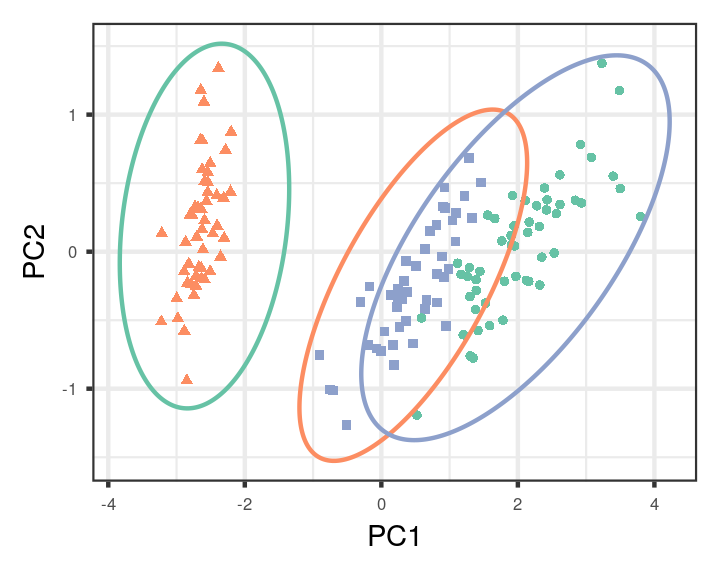
\includegraphics[width=0.588\linewidth,height=0.470\linewidth]{figure/iris_fit-1} 

}

\caption[The iris data in principal component space and
                      GMM fit at $\alpha = 6$.
                      Colors denote inferred memberships and
                      ellipses represent estimated covariances]{The iris data in principal component space and
                      GMM fit at $\alpha = 6$.
                      Colors denote inferred memberships and
                      ellipses represent estimated covariances. }\label{fig:iris_fit}
\end{figure}


\end{knitrout}


% Our posterior quantities,
% the expected number of in-sample clusters and
% the expected number of predictive clusters,
% were defined in~\exref{insample_nclusters, predictive_nclusters}.
% For this application,
% we do not use thresholding in computing the number of clusters
% (i.e. we set $\tau = 0$),
% so we simply write $\gclustersabbr$ and $\gclusterspredabbr$ for the
% in-sample and predictive quantities, respectively.
We formed the linear approximation at the initial
$\alpha_0 = 2$ fit.
Without further optimization, we use the linear approximation
to quickly evaluate
$\etalinglobal(\alpha)$ for a sequence of $\alpha$'s
in the range $\alpha \in [0.1, 4.0]$,
and produce posterior quantities $g(\etalinglobal(\alpha))$.

For this range of $\alpha$,
the predictive quantity appears much more sensitive than
the in-sample quantity (\figref{iris_alpha_sens}).
The in-sample quantity $\gclustersabbr(\etalinglobal(\alpha))$ is nearly constant with value $\approx 3$
(recall that there are three iris species in the data set).
On the other hand, over the same range of $\alpha$,
the predictive quantity $\gclusterspredabbr(\etalinglobal(\alpha))$
varies from
3.0 to
5.6.

Subsequent refits at $\alpha\not=\alpha_0$ confirm the sensitivity conclusions
of our linearized variational parameters.
The values $\g(\etalinglobal(\alpha))$ closely mimic the
values $g(\etaopt(\alpha))$ found by refitting
the variational parameters at each $\alpha$.
Importantly,
the linear approximation is an order of magnitude faster than refitting.
Forming the linear approximation at $\alpha = \alpha_0$,
required 0.02 seconds.
After forming the linear approximation,
computing $\etalinglobal(\alpha)$ for the sequence
of $\alpha$'s considered in \figref{iris_alpha_sens} took another
0.01 seconds.
On the other hand, to refit $\etaopt(\alpha)$ for the set of
$\alpha$s took a total of  9 seconds, with a median refit time of 0.5 seconds.



\begin{knitrout}
\definecolor{shadecolor}{rgb}{0.969, 0.969, 0.969}\color{fgcolor}\begin{figure}[!h]

{\centering 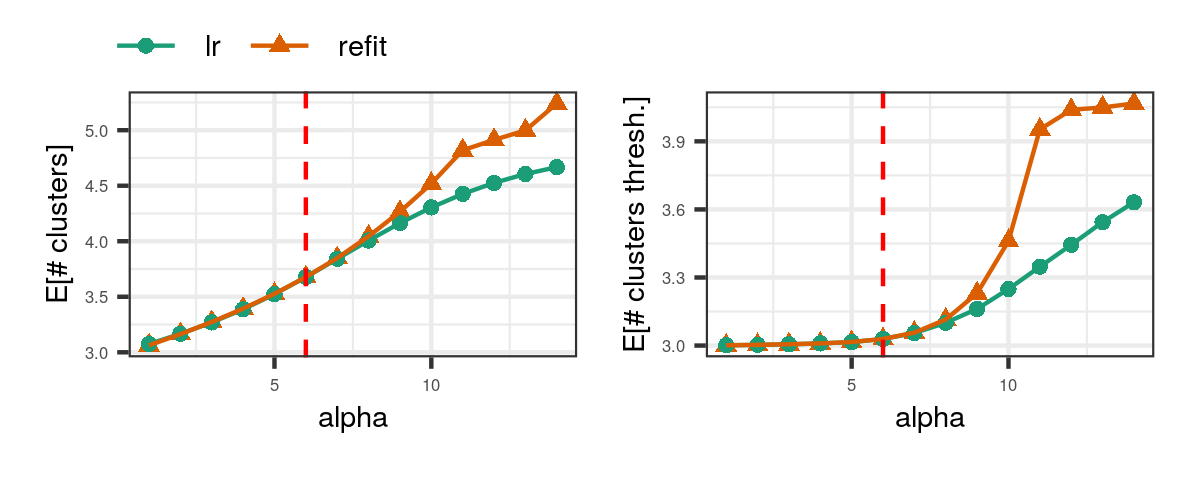
\includegraphics[width=0.784\linewidth,height=0.439\linewidth]{figure/iris_alpha_sens-1} 

}

\caption[The expected number of clusters as $\alpha$ varies in the
the GMM fit of the iris data.
On the left is in-sample quantity $\gclustersabbr$.
On the right is the the predictive quantity $\gclusterspredabbr$.
We formed the linear approximation at $\alpha=2$.
In red, the expected number of clusters computed under the
linearly approximated variational parameters.
In blue, the expected number of clusters obtained by refitting the model at each $\alpha$]{The expected number of clusters as $\alpha$ varies in the
the GMM fit of the iris data.
On the left is in-sample quantity $\gclustersabbr$.
On the right is the the predictive quantity $\gclusterspredabbr$.
We formed the linear approximation at $\alpha=2$.
In red, the expected number of clusters computed under the
linearly approximated variational parameters.
In blue, the expected number of clusters obtained by refitting the model at each $\alpha$. }\label{fig:iris_alpha_sens}
\end{figure}


\end{knitrout}


%
% - we demonstrate the utility of the influence function
% - figure ref top three rows shows three different functional perturbations.
% - can't really tell from densities how these will affect posterior statistic
% - but they do in fact have very different effects (in sign and size).
% - but their effects make sense when looking at the influence function
%
% -last row is worst-case

\subsubsection*{Functional perturbations and the influence function}

We again start with the variational approximation fit with GEM parameter
$\alpha_0 = 2$, but now we consider functional perturbations to
the stick-breaking $\betadist{1, \alpha_0}$ density.
We demonstrate the ability of the influence function to
provide guidance on the anticipated effect of potential perturbations
on the expected number of in-sample clusters.

Recall from \eqref{vb_eta_infl_sens} that the local sensitivity can
be represented as an inner product between the influence function $\infl$
and a multiplicative perturbation $\phi$;
the inner product takes the form,
\begin{align}\eqlabel{recall_infl_innerprod}
\fracat{d g(\etaopt(\t \phi))}{d \t}{0} ={}&
    \int \infl(\lnuk) \phi(\lnuk) \mu(d\lnuk),
\end{align}
where we expressed both the influence function and the perturbation in
unconstrained space, $\lnuk := \log(\nuk) - \log(1 - \nuk)$.
The left column of \figref{iris_fsens} shows the influence function
for the number of in-sample clusters $\gclustersabbr$ in purple.

In order to illustrate this inner product,
we consider perturbations $\phi_\mu$
which are Gaussian bumps, with each perturbation centered at a
different $\mu$ on the real line (\figref{iris_fsens} left column).
The perturbed densities are
$p(\lnu_k|\t\phi_\mu) = p_0(\lnu_k)\exp(\t\phi_\mu(\lnu_k))$.
The middle column of \figref{iris_fsens} displays the initial density
$p_0(\nu_k) = \betadist{\nu_k\vert 1, \alpha_0}$
along with the perturbed densities at $\t = 1$
for different choices of $\mu$,
in the original $(0, 1)$ constrained space.


% The perturbations of the form
% $\phi_\mu(x) = e^{2(x - \mu)^2}$, with each perturbation having a
% different mode $\mu$ (\figref{iris_fsens} left column).
% The perturbations are multiplicative with perturbed prior
% $p(\nu_k|\t) = p_0(\nu_k)\exp(\t\phi_\mu(\nu_k))$.
% The middle column of \figref{iris_fsens} displays the initial density,
% $p_0(\nu_k) = \betadist{\nu_k\vert 1, \alpha_0}$,
% along with the perturbed densities
% $p(\nu_k|\t = 1)$ for different choices of $\mu$.

Each perturbation $\phi_\mu$ with a different choice of $\mu$
produces distinct changes in the expected number
of in-sample clusters $\gclustersabbr$.
The right column of \figref{iris_fsens} plots the differences
$\Delta\gclustersabbr(\eta(\t)) :=
\gclustersabbr(\eta(\t)) - \gclustersabbr(\etaopt(0))$
for $\t\in[0,1]$.
Depending on the perturbation,
$\Delta\gclustersabbr$ can be positive, negative, or nearly zero.
In each case, the approximation
$\Delta\gclustersabbr(\etalinglobal(\t))$
is able to mirror the qualitative behavior of
$\Delta\gclustersabbr(\etaopt(\t))$
observed by refitting.

While each perturbation produces distinct changes in $\gclustersabbr$,
it is unclear how to anticipate the effect of a perturbation
by comparing the original and perturbed densities alone.
On the other hand, the sign and magnitude of the change in $\gclustersabbr$ after
prior perturbation are well-explained by its influence function
and the representation of local sensitivity as an inner product
(\eqref{recall_infl_innerprod}).
When $\phi_\mu$ is centered at a location where the influence function is negative, the effect of the perturbation on $\gclustersabbr$
is negative (\figref{iris_fsens} top row);
conversely, when $\phi_\mu$ is centered at a location where the influence function is positive, its effect on $\gclustersabbr$ is positive (bottom row);
finally, when $\phi_\mu$ is centered at a location where the influence transitions from negative to positive, its effect on
$\gclustersabbr$ is roughly zero (middle row).
In the last case, $\phi_\mu$ placed approximately equal weight on the negative and positive portions of the prior-weighted influence function, resulting in an approximately zero inner-product.


Finally, we consider the
worst-case multiplicative perturbation with unit $L_\infty$ norm.
Recall that the worst-case perturbation with unit $L_\infty$ norm is a
step-function taking on values $\pm1$ corresponding
to the sign of the influence function (\figref{iris_worstcase} left).
The middle column of \figref{iris_worstcase} shows the prior density perturbed by the worst-case perturbation;
the right column shows the effect on $\gclustersabbr$.
This worst-case perturbation has a much larger effect on
$\gclustersabbr$ compared to the other unit $L_\infty$ norm perturbations in
\figref{iris_fsens}.
However, even with the worst-case perturbation,
the change in $\gclustersabbr$ is still small.
We conclude that on the iris data set, $\gclustersabbr$ appears to be a quantity insensitive to the prior under a Gaussian mixture model.



\begin{knitrout}
\definecolor{shadecolor}{rgb}{0.969, 0.969, 0.969}\color{fgcolor}\begin{figure}[!h]

{\centering 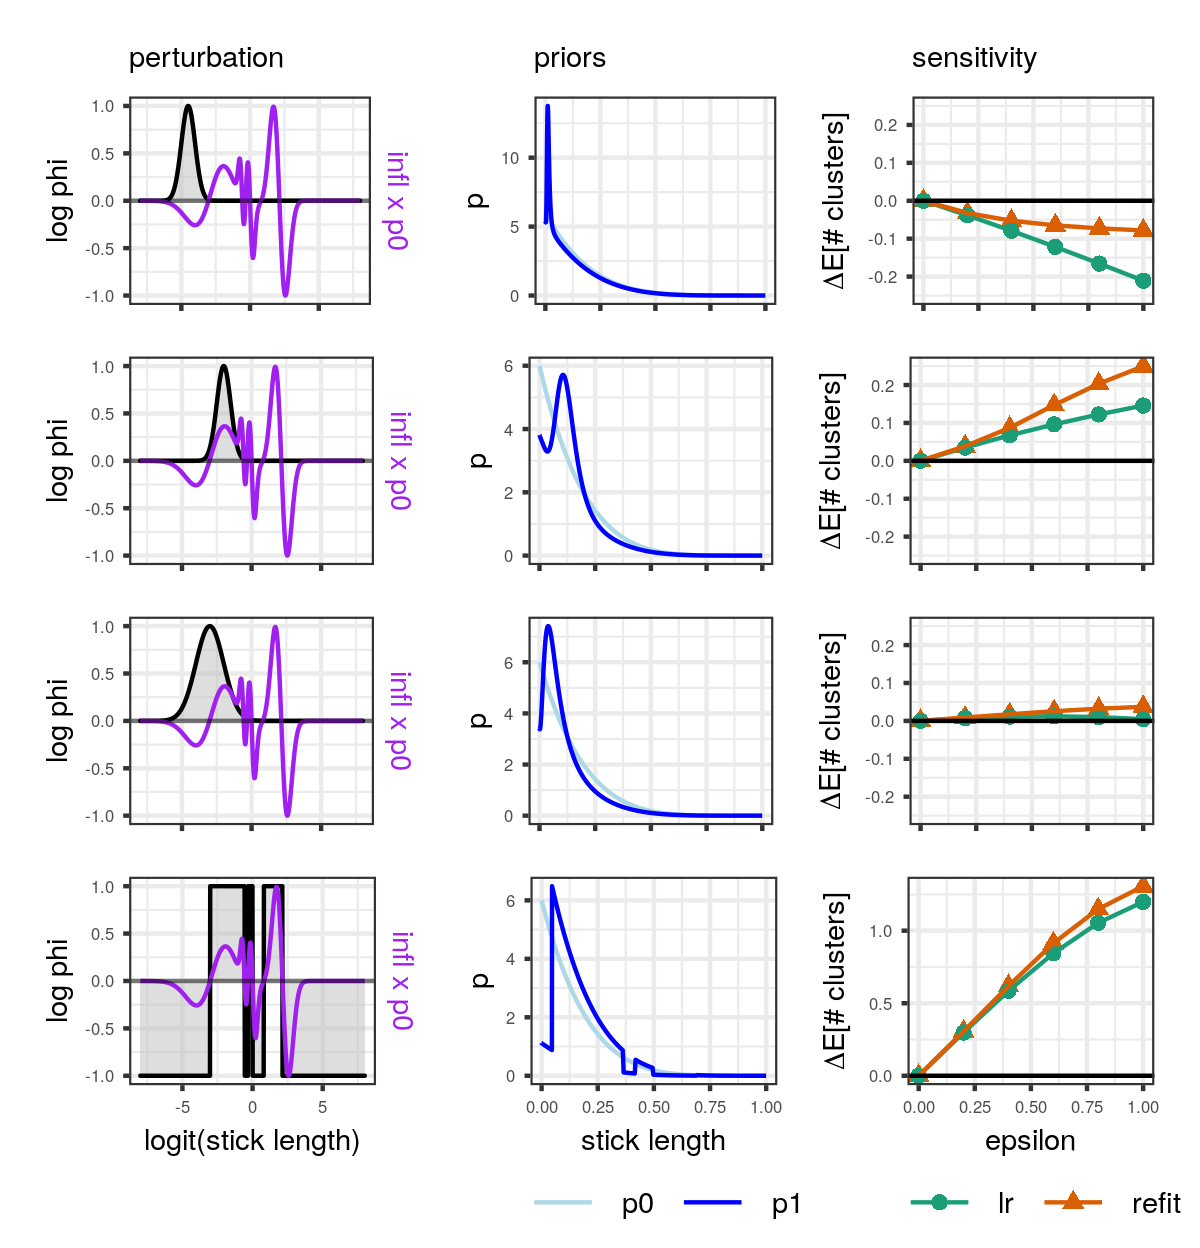
\includegraphics[width=0.980\linewidth,height=0.862\linewidth]{figure/iris_fsens-1} 

}

\caption{Sensitivity of
        the expected number of in-sample clusters
        in the iris data set
        to three multiplicative perturbations with
        unit $L_{\infty}$-norm.
        (Left) the multiplicative perturbation $\phi$ in grey.
        The influence function $\Psi$ in purple,
        scaled to also have unit $L_{\infty}$-norm.
        (Middle) the original prior density $\p_0$ and
        the perturbed prior density $\p_t = \p_0\times \exp(t \phi)$
        at $t = 1$.
        (Right) the effect of the perturbation
        on the change in expected number of in-sample clusters
        as $t\rightarrow1$.}\label{fig:iris_fsens}
\end{figure}


\end{knitrout}


\begin{knitrout}
\definecolor{shadecolor}{rgb}{0.969, 0.969, 0.969}\color{fgcolor}\begin{figure}[!h]

{\centering 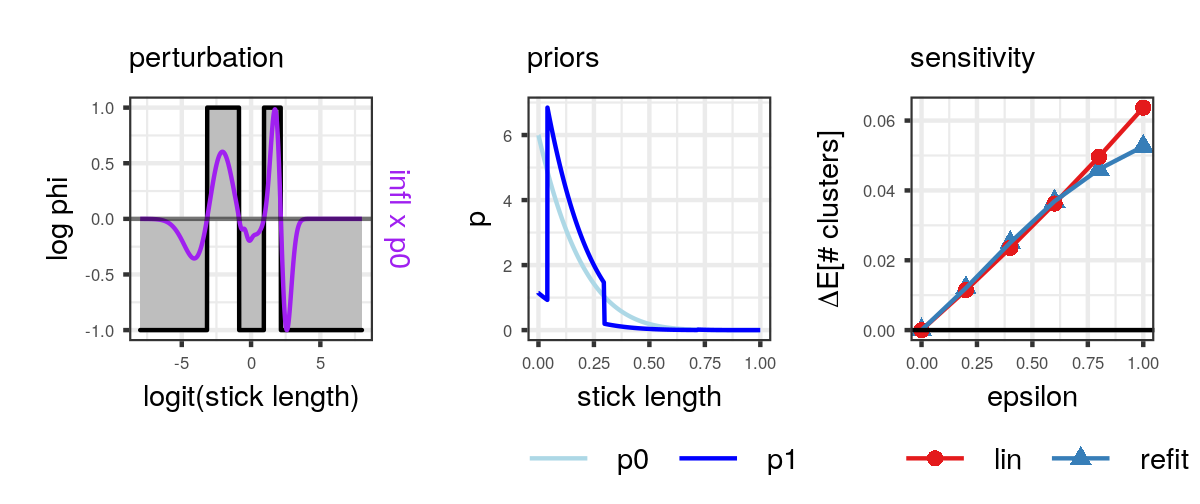
\includegraphics[width=0.980\linewidth,height=0.412\linewidth]{figure/iris_worstcase-1} 

}

\caption[Sensitivity of
        the expected number of in-sample clusters in the iris data set
        to the worst-case multiplicative perturbation with
        unit $L_{\infty}$-norm]{Sensitivity of
        the expected number of in-sample clusters in the iris data set
        to the worst-case multiplicative perturbation with
        unit $L_{\infty}$-norm.}\label{fig:iris_worstcase}
\end{figure}


\end{knitrout}

Computing the linearized variational parameters $\etalinglobal(\t)$ at $\t = 1$
(including the necessary Hessian solve)
for a given functional perturbation
required 0.03 seconds.
A refit at $\t = 1$ requires about one second.
While a second for a refit is not exceedingly large, the
order-of-magnitude difference in timing between the linear approximation and refit
will continue to hold for larger data analysis problems below.
In general, the speed of the linear approximation allows us to quickly
explore many different potential functional perturbations when
refitting for each perturbation becomes prohibitive.
In the data applications below,
the influence function will guide our choice of functional perturbation and
uncover potentially influential perturbations.

% \begin{table}[tb]
% \centering
% \caption{Compute time of results on the iris data set. }
% \begin{tabular}{|r|r|}
%     \hline
%     & time (seconds) \\
%     \hline
%     Initial fit & sprintf('%1.2g', init_fit_time) \\
%     \hline
%     Hessian solve for $\alpha$ sensitivity &
%         sprintf('%1.2g', alpha_hess_time)\\
%     Linear approx. $\eta^{lin}(\alpha)$ for $\alpha = 1, \ldots , 16$ &
%         sprintf('%1.2g', total_alpha_lr_time)\\
%     Refits $\eta(\alpha)$ for $\alpha = 1, \ldots , 16$ &
%         sprintf('%1.2g', total_alpha_refit_time)\\
%     \hline
%     The influence function & sprintf('%1.2g', infl_time)\\
%     Hessian solve for worst-case $\phi$ &
%         sprintf('%1.2g', wc_hessian_time)\\
%     Linear approx. $\eta^{lin}(\t)|_{\t = 1}$
%     for worst-case $\phi$ &
%         sprintf('%1.2g', wc_lr_time)\\
%     Refit $\eta(\t)|_{\t = 1}$ for worst-case $\phi$ &
%         sprintf('%1.2g', wc_refit_time)\\
%     \hline
% \end{tabular}
% \end{table}
